% !TEX encoding = UTF-8 Unicode

% Format teze zasnovan je na paketu memoir
% http://tug.ctan.org/macros/latex/contrib/memoir/memman.pdf ili
% http://texdoc.net/texmf-dist/doc/latex/memoir/memman.pdf
% 
% Prilikom zadavanja klase memoir, navedenim opcijama se podešava 
% veličina slova (12pt) i jednostrano štampanje (oneside).
% Ove parametre možete menjati samo ako pravite nezvanične verzije
% mastera za privatnu upotrebu (na primer, u b5 varijanti ima smisla 
% smanjiti 
\documentclass[12pt,oneside]{memoir} 

% Paket koji definiše sve specifičnosti master rada Matematičkog fakulteta
\usepackage[latinica]{matfmaster} 
%

\usepackage{amsmath}
% \usepackage{color}
% \usepackage{url}
% \usepackage[utf8]{inputenc} % make weird characters work
\usepackage{graphicx}
\graphicspath{{figures/}} %Setting the graphicspath

% \usepackage[english,serbian]{babel}
% \usepackage[english,serbianc]{babel} %ukljuciti babel sa ovim opcijama, umesto gornjim, ukoliko se koristi cirilica

\usepackage[unicode]{hyperref}
\hypersetup{colorlinks,citecolor=green,filecolor=green,linkcolor=blue,urlcolor=blue}

\usepackage{algorithm}
\usepackage{algpseudocode}

%header
% \usepackage{fancyhdr}
% \pagestyle{fancy}

%\newtheorem{primer}{Пример}[section] %ćirilični primer
\newtheorem{primer}{Primer}[section]
\newtheorem{defi}{Definicija}[section]
\newtheorem{teo}{Teorema}[section]

% Datoteka sa literaturom u BibTex tj. BibLaTeX/Biber formatu
\bib{master}

% Ime kandidata na srpskom jeziku (u odabranom pismu)
\autor{Nikola Dimitrijević}
% Naslov teze na srpskom jeziku (u odabranom pismu)
\naslov{Detekcija kolizije u realnom vremenu}
% Godina u kojoj je teza predana komisiji
\godina{2019}
% Ime i afilijacija mentora (u odabranom pismu)
\mentor{dr Vesna \textsc{Marinković} \\ Univerzitet u Beogradu, Matematički fakultet}
% Ime i afilijacija prvog člana komisije (u odabranom pismu)
\komisijaA{dr Predrag \textsc{Janičić } \\ Univerzitet u Beogradu, Matematički fakultet}
% Ime i afilijacija drugog člana komisije (u odabranom pismu)
\komisijaB{dr Ivan \textsc{Čukić} \\ Univerzitet u Beogradu, Matematički fakultet}
% Datum odbrane (odkomentarisati narednu liniju i upisati datum odbrane ako je poznat)
\datumodbrane{ }

% Apstrakt na srpskom jeziku (u odabranom pismu)
\apstr{%
 Rezime.
}

% Ključne reči na srpskom jeziku (u odabranom pismu)
\kljucnereci{kolizija, grafika, računarstvo, algoritmi}

\begin{document}
% ==============================================================================
% Uvodni deo teze
\frontmatter
% ==============================================================================

% Naslovna strana
\naslovna
% Strana sa podacima o mentoru i članovima komisije
\komisija
% Strana sa posvetom (u odabranom pismu)
% \posveta{Mami, tati i dedi}
% Strana sa podacima o disertaciji na srpskom jeziku
\apstrakt
% Sadržaj teze
% \pagenumbering{arabic}
\tableofcontents*

\mainmatter

% ==============================================================================
\chapter{Uvod}
\label{sec:uvod}
% ==============================================================================

Uvod.

\section{Motivacija}
\label{sec:naslov1}
Detekcija kolizije ima široke primene uključujući virtuelnu realnost, računarske igre, planiranje putanje robota i
fizičke simulacije.
Detekcija kolizije u realnom vremenu je ključan deo svakog pogona igre (eng. {\em game engine}), a danas ga svaka velika
video igra koristi. Industrija video igara svake godine raste \cite{game_industry},
toliko da ima veći prihod od filmske i muzičke industrije zajedno! Zaista, industrija igara ima prihod od
115 milijardi dolara naspram 41 milijardi filmske i 17 milijardi muzičke industrije \cite{music} \cite{movie} \cite{game_industry}.
Posledice neispravnosti igara nisu dramaticne poput neispravnost softvera u avionskoj ili automobilskoj industriji, ali 
se svakako jasno odražavaju negativno na prihod.
Korisnici očekuju visok stepen doteranosti video igara, pa bi postojanje velikog broja bagova 
 obeshrabrilo potencijalne kupce. Na slici \ref{fig:batman} se vidi bag gde je igrač propao kroz 
 mapu, a na slici \ref{fig:horse} igrač ne može da se popne na konja pošto on lebdi u vazduhu.

Pojavljuju se na tržištu VR rukavice koje simuliraju dodir virtuelnih objekata, a za njih je 
detekcija kolizije svakako presudna. Potrebno je bar 1000 puta u sekundi pružiti povratnu informaciju
da bi simulacija dodira bila uverljiva \cite{haptic}. 

\begin{figure}[h!]
\centering
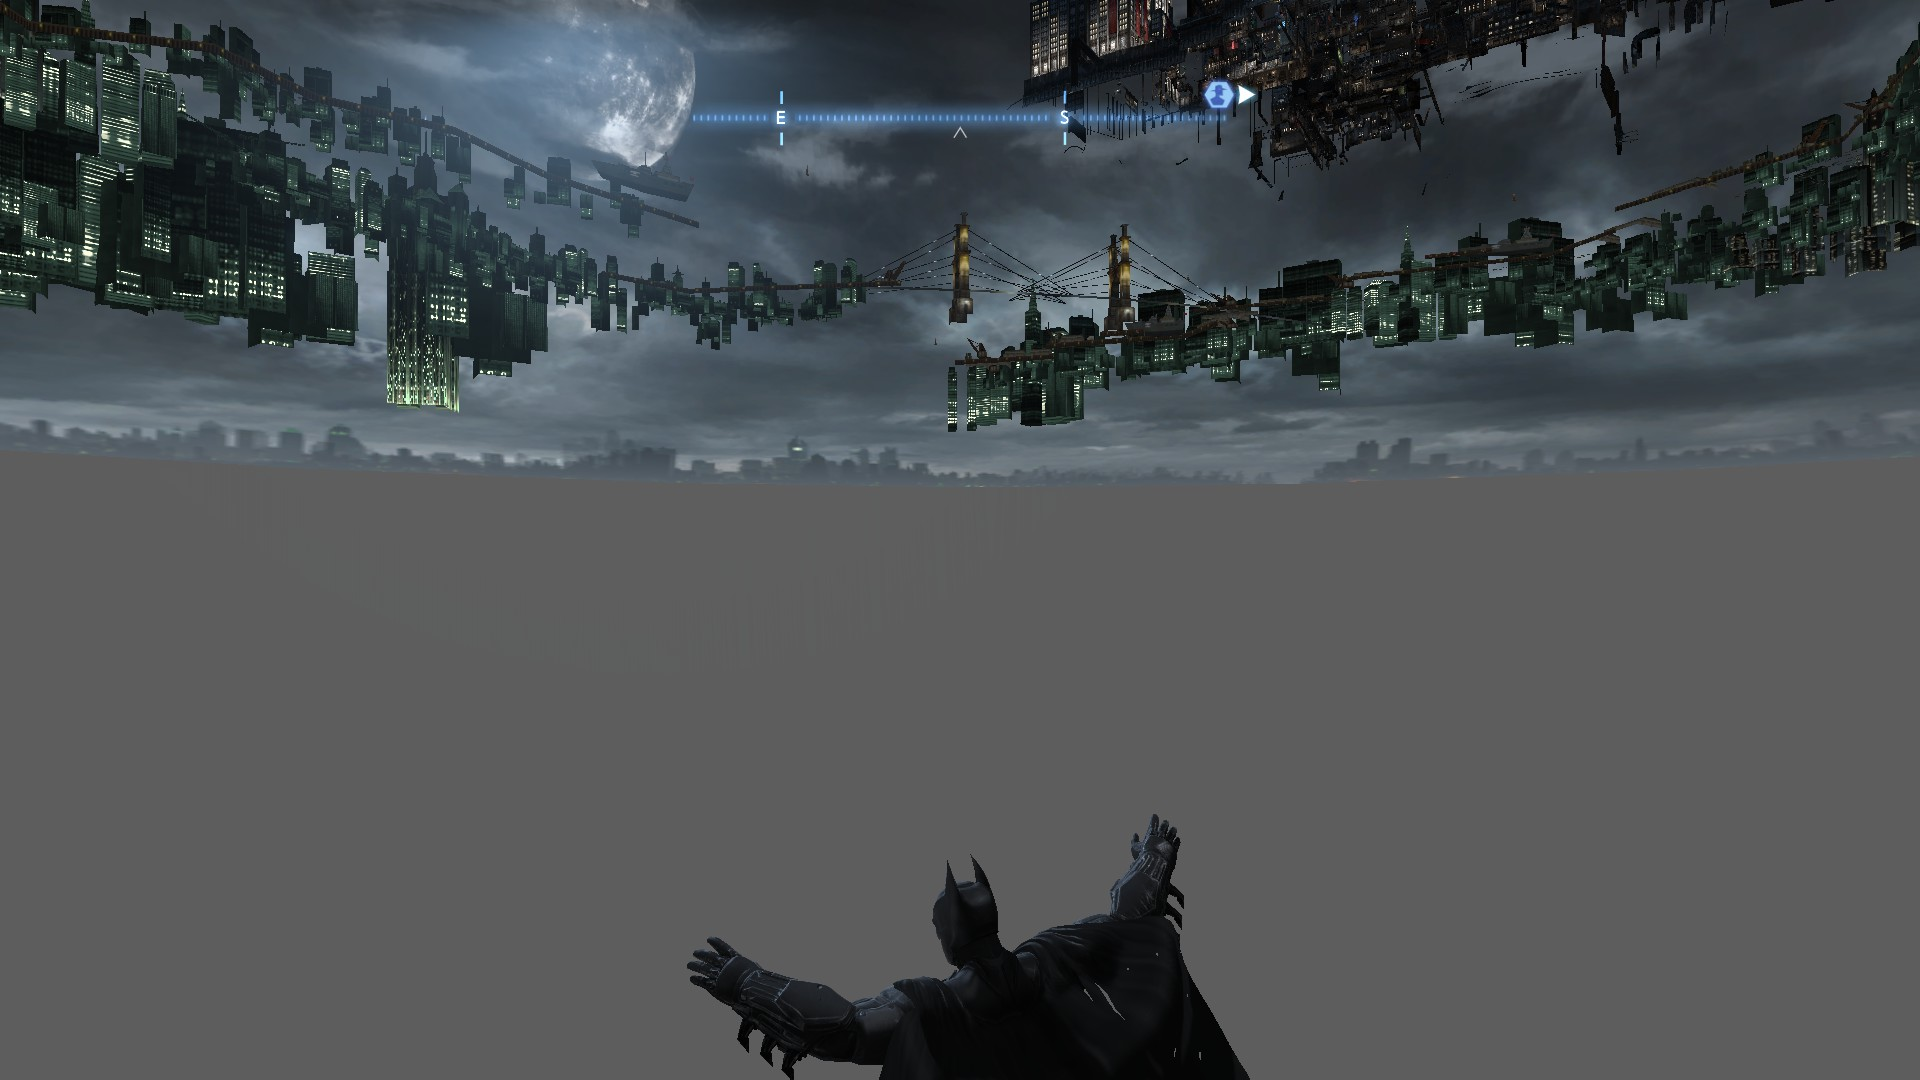
\includegraphics[scale=0.22]{batman.jpg}
\caption{Propadanje kroz mapu.}
\label{fig:batman}
\end{figure}

\begin{figure}[h!]
	\centering
	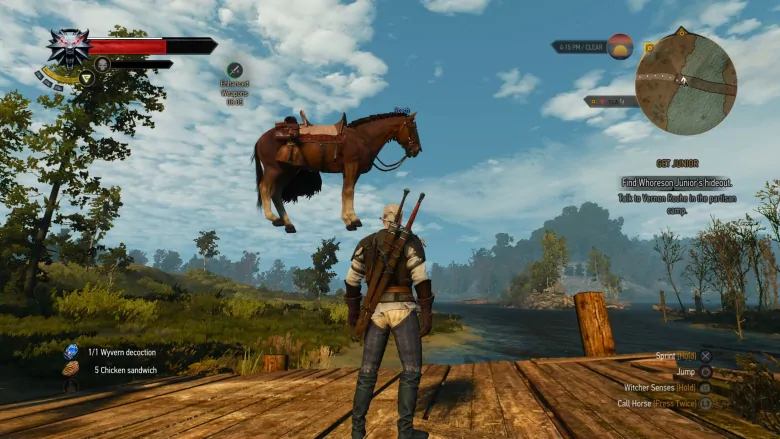
\includegraphics[scale=0.54]{horse.png}
	\caption{Levitirajući konj.}
	\label{fig:horse}
\end{figure}

Problem detekcije svih parova kolizije je u najgorem slučaju kvadratne složenosti i od toga se ne može pobeći,
ali uglavnom ih ima mnogo manje od gornje granice.
Razlog zahteva da se izvršava u realnom vremenu kod interaktivnih programa je očigledan, ali je takođe
potrebana mogućnost da se što češće i efikasnije utvrde kolizije. Filmovi nisu interaktivan sadržaj i zato
je učestalost osvežavanja slike od 24hz, uz korišćenje zamućivanja pokreta (eng. {\em motion blur}),
dovoljno dobro za većinu ljudi. Standard za igre na konzolama je barem 30hz, a na desktop računarima 
cilj je barem 60hz. Za VR je potrebno barem 90hz inače će lako prouzrokovati dizorijentaciju, mučninu i druge
neželjene efekte \cite{importance}.

Nema najboljeg algoritma detekcije kolizije za svaki mogući slučaj. 
Neki su dobri za uniformno raspoređene objekte u prostoru, ali loši kada su svi na jednom mestu, 
dok su drugi indiferentni što se tiče raspršenosti i više im je bitna brzina kretanja objekata.
Takođe, isti algoritam može imati značajno bolje performanse ako su njegovi parametri dobro 
izabrani za neku hardversku arhitekturu ili scenario. 
Te okolnosti su inspirisale razvoj programa koji omogućava brzo i interaktivno menjanje različitih
algoritama detekcije kolizije, postavljanje njihovih parametara kao i posmatranje performansi.

% ==============================================================================
\chapter{Glavne karakteristike}
\label{sec:karakteristike}
% ==============================================================================

\section{Faze}
Broadphase, narrowphase, bounding box.

Celokupan zadatak detekcije kolizije se deli na dve faze: broadphase i narrowphase. 
U prvoj fazi, broadphase, odbacuje se vecina kandidata mogucih parova koji imaju koliziju, i cilj je da 
da faza bude sto efikasnija u odnosu na broj svih elemenata.
Iako postoje slučajevi, u mnogim primenama nisu svi objekti prosta geometrijska tela poput kocki, kvadara ili lopti.
Mogu biti razna kompleksna tela poput kompozicije prostijih tela, ili trijangulisana reprezentacija 
nekih objekata. Ta kompleksnija tela mogu biti sastavljena od velikog broja tih prostijih delova ili
od stotina hiljada trouglova. Tada bi bilo vrlo neefikasno i nepraktično tražiti kolizije posmatrajući
tako kompleksne strukture objekata. Mnogo je bolje da se razmatra nekakva jednostavnija reprezentacija svih 
tih objekata. Ono što se najčešće radi jeste da se naprave najmanje kutije koje će sadržati u potpunosti te objekte.
Te kutije su u obliku kvadra i svaka njegova strana je paralelna nekoj osi koordinatnog sistema. 
Umesto da se računaju preseci između velikog broja prostih objekata koji čine celinu jednog, sada se posmatraju 
samo preseci među kutijama koje sadrže sve objekte. Taj metod se naziva ograničavajuće kutije
porvnane prema osama (eng. {\em Axis Aligned Bounding Box}), odnosno AABB.

todo moguće je i sfera, orijentisan Bounding box, convex hull.

\begin{teo}
	Teorema o razdvajajućim osama. 

	Dva konveksna objekta se ne preklapaju ako postoji prava (osa) na kojoj se projekcije 
	tih objekata ne preklapaju. 
\end{teo}
Nezavisno od dimenzionalnosti, razdvajajuća osa je uvek linija. Na primer, trodimenzionalan prostor
je razdvojiv ravnima, ali razdvajajuća osa je normalna na razdvajajuću ravan.

Teorema o razdvajajućim osama daje inspiraciju za konstrukciju algoritma provere kolizije.
Dovoljno je pronaći samo jednu pravu tako da se  projekcije tela na njoj ne preklapaju.
Moguće je na primer da se uzmu normalne svih lica jednog trijangulisanog tela, izračunaju projekcije drugog 
tela na svaku pravu, i ako postoji neka prava na kojoj ne postoji presek onda uopste i nema preseka između
dva tela. Međutim to nije dovoljno dobro za potrebe detekcije kolizije u realnom vremenu. Zato se tokom 
broadphase ova teorema primenjuje samo za proveru preseka među AABB.

Teorema o razdvajajućim osama je takođe korisna za pronalaženje minimalnog vektora translacije, odnosno
vektor najmanjeg intenziteta za koji treba jedan objekat da se pomeri da bi prestalo da bude kolizije među dva objekta.
Minimalni vektor translacije je vrlo koristan prilikom razrešavanja kolizije, odnosno kada se ustanovi da
se dva objekta prekpapaju, potrebno je pomeriti ih tako da se više ne seku i promeniti im vektore brzina.
Međutim to je posao koji je odvojen od problema detekcije kolizije pa neće biti mnogo dublje razmatran.

Kada se ustanovi da postoji presek između dve AABB, to ne znači da zaista postoji presek između dva objekta
koje ti AABB enkapsuliraju. Na primer, jedan AABB može da sadrži loptu prečnika $r$, a drugi 
da sadrži objekat sagraćen od tankih ivica kocke čija je dužina ivice $r$. Tada se zaista njihove kutije 
seku, iako tela unutar njih nemaju presek.

todo slika

%https://www.scss.tcd.ie/~manzkem/CS7057/cs7057-1516-07-NarrowPhase-mm.pdf
Rešavanje problema određivanja da li postoji presek objekata unutar AABB koji su kandidati za koliziju 
se radi u narrowphase fazi. Bounding volume hierarchies, AABB tree, OBB tree.


U slučaju da su ti objekti unutar AABB neka prosta geometrijska tela poput
lopte ili kvadra, tada možemo lako primeniti teoremu o razdvajajućim osama da bismo videli da li zaista 
postoji preklapanje među njima. Međutim, krije se jedan problem.
AABB se mogu posmatrati kao projekcije tela na sve tri ose u prostoru.
Tada se dakle posmatraju samo tri prave, ne sve moguće prave. 
U slučaju prikazanom na "slici" ispod, vidi se krug i rotiran pravougaonik. Ako gledamo njihove projekcije 
na $x$ i $y$ ose onda oni prema tome imaju presek, iako posmatrajući sliku očigledno nema preseka.
Pomoću opisanog kontraprimera se vidi da posmatranjem projekcija na samo bazne ose prostora nije dovoljno
u opštem slučaju. Na slici \ref{fig:counter} prikazana su dva oblika, jedan konveksan a drugi nekonveksan. 
Za bilo koju pravu projekcija oblika na nju ima presek, iako oni u stvari nemaju presek, što predstavlja 
primer razloga zašto teorema o razdvajajućim osama zahteva konveksna objekta.

\begin{verbatim}
todo slika

\-\
 \ \
O \_\
\end{verbatim}


\begin{figure}[h!]
	\begin{center}
	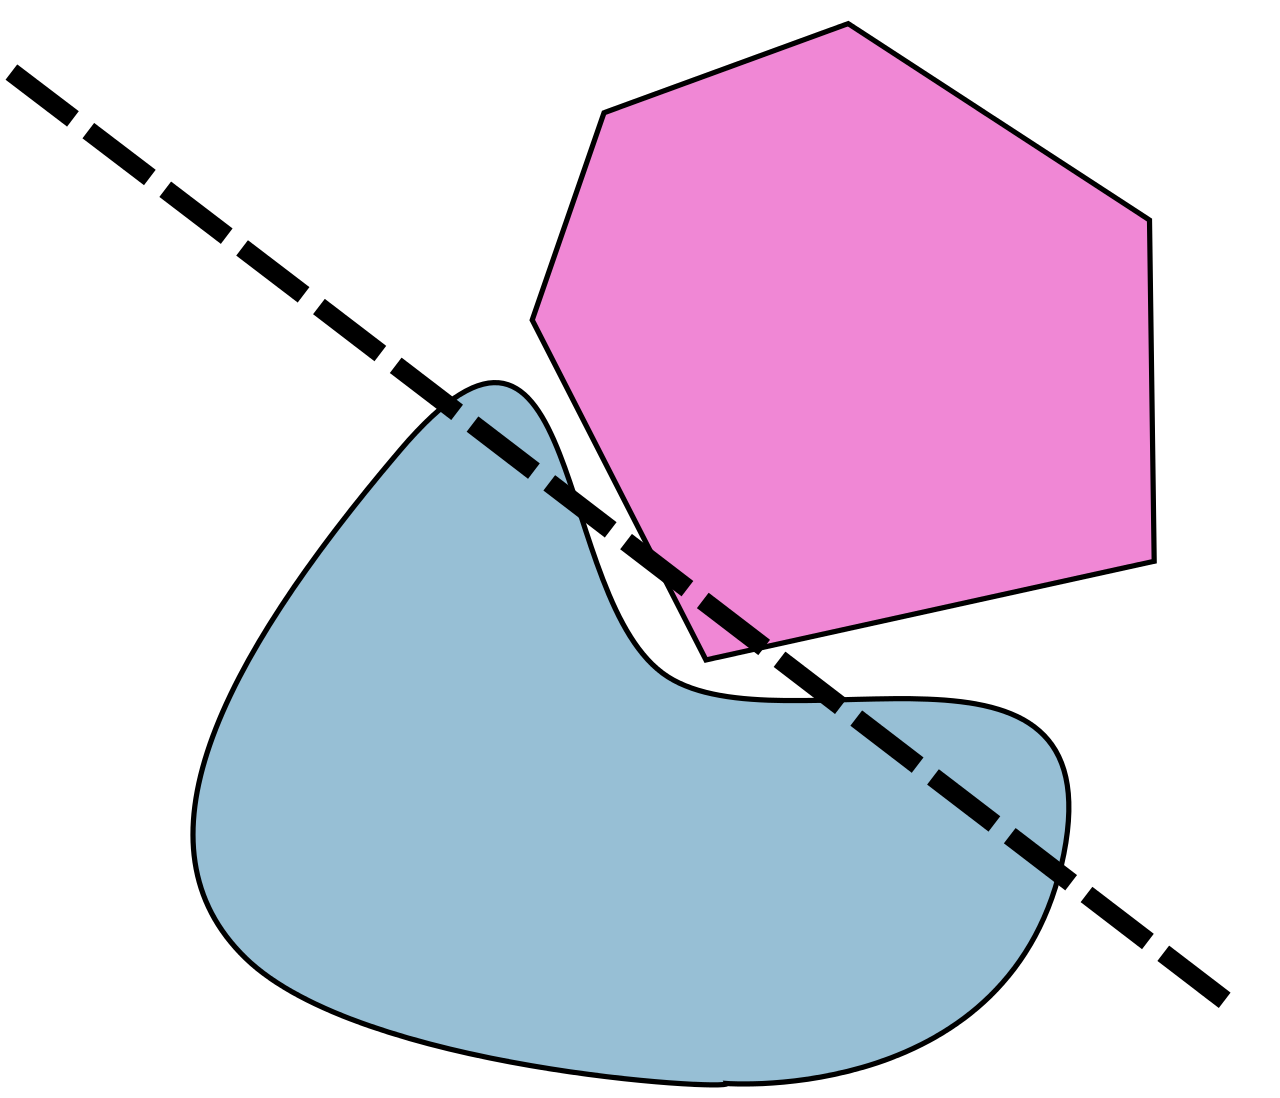
\includegraphics[scale=0.2]{theorem_counterexample.png}
	\end{center}
	\caption{Projekcija nekonveksne površi na pravu.}
	\label{fig:counter}
\end{figure}

\section{Konzistentnost vremena izvršavanja}

Nekad je od interesa samo ukupno vreme potrošeno za više iteracija provere kolizije.
To svakako nije slučaj za potrebe izvršavanja u realnom vremenu. Ako samo jedna iteracija 
detekcije kolizije traje višestruko duže od ostalih onda dolazi do takozvanog "seckanja" što
kad se dešava  u prevelikoj meri dovodi do neupotrebljivog proizvoda pošto korisnicima postaje nepodnošljivo
korišćenje takvog programa.
Opisan problem je jasan i očekivano je da se to želi izbeći. 
Međutim sledi sličan problem koji nije očigledno da toliko smeta.
Ekrani imaju fiksnu učestalost osvežavanja, najčešće je 60hz, mada postaju sve više popularni 
% https://www.blurbusters.com/faq/120hz-monitors/
ekrani sa 120, 144, pa čak i 240hz učestalošću osvežavanja. Dakle ekran od 60hz će svakih 
16.67 milisekundi iscrtati sledeću sliku. Ako se između dva osvežavanja ekrana uvek pripremi
nova slika to je odlično. 
Još bolje da nova slika bude izračunata neposredno pre osvežavanja ekrana jer se onda 
prikazuje verodostojnija slika za taj trenutak. 
Svakako će uvek postojati neko kašnjenje od trenutka interakcije korisnika sa igrom ili simulacijom do
trenutka kada se prikaže slika, ali je cilj da to kašnjenje bude što manje. 
Kada se u jednom ciklusu osvežavanja ekrana pripremi više od jedne slike, onda se uzima ona koja je najnovija,
a prethodne se odbacuju. 
Dakle praktično je bačen trud uložen u pravljenje svih slika osim poslednje.
Kada nije izračunata nova slika za sledeći ciklus osvežavanja ekrana onda će opet biti prikazana slika
iz prošlog ciklusa. Tada se gubi maksimalna glatkoća slike i brzina odziva programa. 
Broj slika po sekundi (eng. {\em Frames per second}), FPS, je broj slika koje program napravi u jednoj sekundi.
Naizgled ako program ima 60FPS to je savršeno za ekran od 60hz. To ipak ne mora da bude slučaj.
U toku jedne sekunde u prvih 500 milisekundi može biti 59 slika, a u preostalih 500 milisekundi samo jedna 
nova slika. To zaista jeste 60FPS, ali ono što je prikazano na ekranu nije mnogo bolje od 2FPS,
što je prektično uvek nedopustivo loše. 
Dakle sa jedne strane nije dobar višak slika jer se nepotrebno troše resursi na njih iako se ne prikazuju, 
a sa druge strane manjak slika dovodi do neprijatnosti.
Zato je bitno da cela simulacija, a samim tim i detekcija kolizije ima što konzistentnije vreme izvršavanja.

Na slici <todo> se vidi da je program napravio 60 slika, tj. da praktično ima 60fps, iako je prikaz na ekranu 
ekvivalentan sa 30FPS, što je još jedan primer nepoželjne posledice nekonzistentnosti vremena izvršavanja. 

todo nacrtaj sliku gde su svaki parni trenutak osvežavanja ekrana sadrži dva frejma, a svaki neparni 
nijedan


\section{Temporalna koherencija}

Često nije cilj samo jednom odrediti kolizije za neku scenu, nego i kolizije u trenutku koji ubrzo sledi.
Objekti na sceni se u glavnom ne teleportuju nego se malo po malo kreću sa prolaskom vremena.
Tako su pozicije objekata u bliskim trenucima slični i to se može iskoristiti za dodatno ubrzanje algoritama 
detekcije kolizije. Generalno je princip da se čuvaju svi parovi kolizije i u svakoj iteraciji 
izbace oni oni koji više nisu u koliziji a dodaju oni koji su u tom trenutku došli u koliziju.
Na taj način se značajno smanjuje vreme potrebno za izračunavanje kolizija kroz iteracije.
U slučaju da se objekti jako sporo ili uopšte ne kreću algoritmi koji dobro koriste svojstvo temporalne 
koherencije će u svakoj iteraciji imati linearno vreme izvršavanja, što će posle biti dublje razmatrano. 


\section{Temporalni anti-aliasing}

Temporalni anti-aliasing ima za cilj da smanji ili ukloni efekte temporalnog aliasinga.
Temporalni aliasing nastaje zbog premalog broja slika u sekundi u poređenju sa brzinom kretanja objekata na sceni.
Zbog toga objekti izgledaju kao da poskaču  umesto da odaju utisak glatkog kretanja.
Da bi se izbegao temporalni aliasing potrebno je da broj slika scene u sekundi bude bar duplo veći 
od objekta koji se najbrže kreće \cite{Grant}. Čest primer temporalnog aliasinga je da se na snimku točkovi naizgled 
kreću unazad.
Temporalni anti-aliasing se takođe koristi za smanjenje oštrih ivica koje trepere kada se pomera kamera.
Na slici \ref{fig:txaa} se vidi jasno poboljšanje kada se koristi TXAA, što je temporalni anti
aliasing firme NVIDIA.

\begin{figure}[h!]
	\begin{center}
	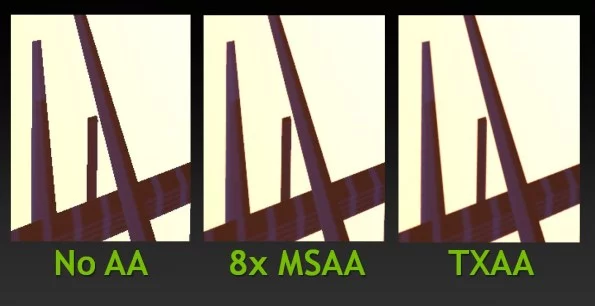
\includegraphics[scale=0.65]{txaa.png}
	\end{center}
	\caption{Upoređivanje tehnika anti-aliasinga.}
	\label{fig:txaa}
\end{figure}

\section{Preciznost, preseci zapremina pokretnih tela.}

Moguće su različite preciznosti detekcije kolizije. 
Uglavnom je razlog za odabir nepreciznije opcije kraće vreme izvršavanja i manja potrošnja memorije.
Pošto se provera kolizije dešava u diskretnim vremenskim trenucima umesto kontinualno, onda je moguće da 
je između dva uzastopna trenutka bilo kolizije, iako u nijednom od njih nema kolizije. 
Ovaj fenom se naziva tuneliranje (eng. {\em. tunneling}) i prikazan je primer na slici \ref{fig:tunnel}. 

\begin{figure}[h!]
	\begin{center}
	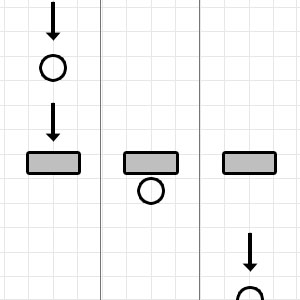
\includegraphics[scale=0.55]{tunnel.png}
	\end{center}
	\caption{Tuneliranje.}
	\label{fig:tunnel}
\end{figure}

Tuneliranje se češće dešava kod malih objekata, a takođe i kod 
onih koji se brzo kreću. U oba slučaja problem je u tome što je put koji objekat pređe između dve provere 
kolizija velik u odnosu na veličinu objekta. 
Problem se rešava tako što se ne proverava kolizija za sâm objekat, već za celu zapreminu kroz koju je on prošao 
od prošlog trenutka provere kolizije pa do trenutnog. Na slici \ref{fig:tunnel_fix} je obojena zapremina 
koja se dodatno proverava umesto samo zapremine objekta.



\begin{figure}[h!]
	\begin{center}
	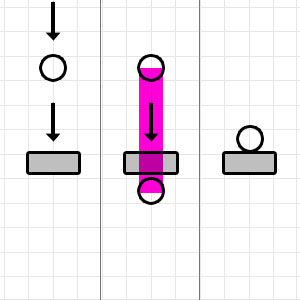
\includegraphics[scale=0.55]{tunnel_fixed.png}
	\end{center}
	\caption{Sprečavanje tuneliranja.}
	\label{fig:tunnel_fix}
\end{figure}

Pod preciznošću se može smatrati i verodostojnost među grafičkim modelima i objektima koji predstavljaju njihovu koliziju.
Na slici \ref{fig:hitbox} je prikazana aproksimacija kompleksnijeg modela čoveka pomoću manjeg broja kvadara.
Na taj način se može dobiti prostiji, ali dovoljno dobar model za detekciju kolizije koji je značajno 
jeftiniji za upotrebu u realnom vremenu. 

\begin{figure}[h!]
	\begin{center}
	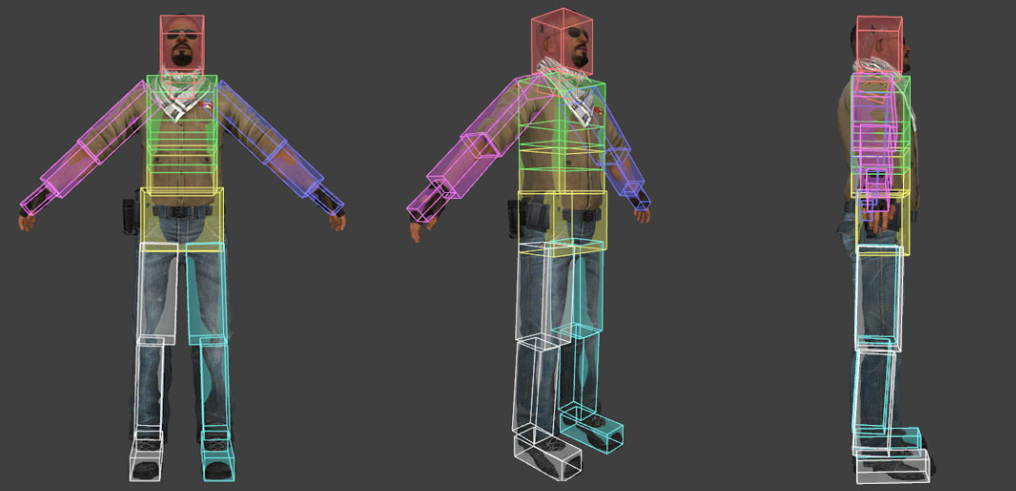
\includegraphics[scale=0.55]{hitbox.png}
	\end{center}
	\caption{Reprezentacija modela čoveka.}
	\label{fig:hitbox}
\end{figure}

\section{Kako radi na različitim konfiguracijama}

Simulacija se izvršava u diskretnim koracima, ali je pitanje kolika je vremenska razlika između dva koraka.
Prevelika razlika između dva koraka je svakako nepoželjna jer je onda i prevelika razlika između dve slike scene.

Na primer, potrebno je objekat pomerati udesno za 10 jedinica svake sekunde. Neka je interval koraka simulacije 
$p$ jednak $0.01$ sekund, onda je dovoljno da se u svakom koraku vrednost x koordinate tog objekta ažurira na sledeći način:

\begin{primer}
\label{pr:x}

$$ x:= x + 10 * 0.01 $$
\end{primer}

Zaista, kako se svakog koraka x uveća za 0.1, a ima tačno 100 koraka u sekundi, onda će se $x$ uvećati za 10 svake sekunde.

Poželjno je da su koraci što bliže, međutim ako bi se izabrao fiksan interval koraka $p$, onda se može desiti
da se na određenoj konfiguraciji sistema program ne izvršava dovoljno brzo. 
Tada bi razlika između dva koraka bila $q$ gde je $q > p$, a u svakom koraku bi simulacija napredovala za 
$p$ jedinica unapred. Kako je $q > p$ onda bi simulacija izgledala kao usporeni snimak.

Rešenje je da se koristi razlika vremena proteklog između dva uzastopna koraka, u oznaci $dt$, (eng. {\em delta time}).
Korišćenjem $dt$ je moguće izvršavanje simulacije čije vreme teče konzistentno nezavisno od broja izvršenih koraka u 
jedinici vremena. Ako je harver bolji onda će imati više koraka, odnosno više slika u sekundi, a ako je 
sporiji onda će biti manje slika u sekundi ali neće izgledati kao da je usporen snimak.
$dt$ bi u idealnom slučaju bio inverz od fps, tj. $dt = 1/fps$, ali proteklo vreme između dve slike je promenljivo.
Može se primetiti da dodvanjam promenljivoj $x$ vrednost $dt$ svakog koraka, u stvari se vrednost $x$ povećava 
za 1 svake sekunde, jer vreme svih koraka tokom jedne sekunde mora ukupno biti baš 1.
Umesto ažuriranja kao u primeru \ref{pr:x}, sada se vrednost $x$ ažurira na sledeći način:
\begin{primer}
	\label{pr:x2}
	
	$$ x:= x + 10 * dt $$
\end{primer}

Kada se koristi $dt$ za ažuiriranje svih objekata onda se lako može simulacija ubrzati množenjem $dt$ 
sa $k$ za $k$-tostruko ubrzanje, ili deljenjem sa $k$ za $k$-tostruko usporenje. Postavljanjem $dt$ na 0 svi 
objekti postaju statični. 
Na vrlo niskim fps igre postaju neprijatne za korišćenje, ali čak mogu postati nestabilne. Dolazi do nepoželjnih efekta 
poput tuneliranja prikazanog na slici \ref{fig:tunnel}. Tada se često uzima donja gornja granica za $dt$, pa 
ako je vreme između dva koraka veće od te gornje granice onda će igra biti u usporenom snimku, što se i želelo izbeći 
ali je često bolji rezultat nego problem tuneliranja.

Pogon igara Unity deli sva ažuriranja na dve vrste: FixedUpdate i Update. 
FixedUpdate se koristi za promene sila nad objektima pošto se koraci izračunavanja fizike izvode u fiksnim intervalima, 
dok se Update koristi za operaicje koje je potrebno izvršiti pre svakog iscrtavanja slike. 
Na primer, izmene korisničkog interfejsa igre spada pod Update, a primena sile ili obrtnog momenta spada pod FixedUpdate.
Unity izvršava FixedUpdate i fiziku 50 puta u sekundi, nezavisno od broja slika u sekundi \cite{unity}.
To znači da ako se igra izvršava na 25fps onda će otprilike biti dva poziva FixedUpdate po svakoj slici,
a ako se izvršava na 100 fps tada između nekih slika neće biti nijednog poziva fizike i FixedUpdate.

\section{Razrešenje kolizije}

Prilikom razrešenja kolizije zadatak je da se pomere objekti tako da se više ne seku i
da se postave njihovi novi vektori brzina i ubrzanja nakon kolizije.
Nakon što algoritam detekcije kolizije odredi sve parove koji su u koliziji, 
posmatranjem svakog para se radi razrešenje kolizije svih objekata.
Postoje dva glavna načina za razrešenje kolizija \cite{Moore}.
Jedan način je da se ubaci kruta opruga između dva objekta u koliziji.
Sila opruge se primenjuje jednako u suprotnom smeru na ta dva objekta.
Smer sile je takav da što pre razdvoji objekte. Metod sa oprugama nije težak 
za implementaciju, dobar je i za tvrda tela i za fleksibilna, ali je problem što je 
računski zahtevan. Što je kruća opruga potrebni su kraći vremenski koraci za fina 
numerička izračunavanja.

Drugi način je da se analitički izračunaju nova svojstva objekata u jednom koraku.
Prvo se izračuna minimalni vektor translacije. Npr. za dve sfere $s_1$ i $s_2$ to je vektor $\vec{m}$
određen centrima $c_1, c_2$ dve sfere čiji je intenzitet jednak razlici intenzitata zbira poluprečnika
$r_1, r_2$ dve sfere i intenziteta udaljenost centara, odnosno:
\[  \vec{m} := \frac{{c_1 - c_2}} {\|{c_1 - c_2}\|} 
 (r_1 + r_2 - \| {c_1 - c_2} \| ) \]
Potom se jedna sfera translira za $ \frac{ \vec{v} }{ 2 }$, a druga za $ -\frac{ \vec{v} }{ 2 }$.
Sada sfere više nisu u koliziji, ali je potrebno da se promene njihovi vektori brzina nakon sudara.
Kada se koristi elastična kolizija onda se računaju prema formulama:

$$  {v}'_1= {v}_1-\frac{2 m_2}{m_1+m_2} \ \frac{\langle  {v}_1- {v}_2,\, {c}_1- {c}_2\rangle}{\| {c}_1- {c}_2\|^2} \ ( {c}_1- {c}_2) $$

$$  {v}'_2= {v}_2-\frac{2 m_1}{m_1+m_2} \ \frac{\langle  {v}_2- {v}_1,\, {c}_2- {c}_1\rangle}{\| {c}_2- {c}_1\|^2} \ ( {c}_2- {c}_1) $$

pri čemu su $m1$ i $m2$ mase lopti.
Analitičko izračuavanje je glavni metod koji se koristi u pogonima igara.
On je pogodniji za jake sudare, pošto je dovoljno jednom izračunati sve promene.
Ipak, za nežnije kolizije poput tela koje je polegnuto na drugo, bolje je koristiti opruge.

% ==============================================================================
\chapter{Odabrani algoritmi}
\label{sec:algoritmi}
% ==============================================================================

Rezultat izvršavanja algoritma detekcije kolizije je skup svih parova koji su u koliziji.
U najgorem slučaju (na primer kada su svi objekti kocke na istoj poziciji) se svaki objekat
seče sa svim ostalim i tada ima $ {n\choose 2}  $ preseka. Međutim, taj najgori slučaj se retko dešava
u stvarnim primenama, pa postoji mnoštvo algoritama detekcije kolizije čija složenost zavisi i od broja
parova koji su u koliziji. Za takave algoritme kažemo da su izlazno-zavisni, tj.
vreme izvršavanja zavisi i od veličine izlaza. Tokom razmatranja algoritama podrazumeva se da su svi
objekti ograničavajuće kutije koje su paralelne osama, tj. AABB.
Broj kolizija među elemntima će dalje biti označen kao $R$. 

\section{Trivijalni algoritam}
\label{subsec:triv}

Intuitivno se može doći do trivijalnog algoritma detekcije kolizije. 
Jednostavno se svaki za element proveri da li ima presek sa svim ostalim elementima.
Algoritam je ispravan i njegova vremenska složenost je $\Theta (n^2) $, dok je prostorna složenost
$O(n^2)$, odnosno $\Theta(R)$, pošto svaki par objekata koji je u koliziji treba sačuvati.
Glavna mana ovakvog algoritma je kvadratna vremenska složenost čak i kada nema nijedne kolizije.
Bolji algoritmi rešavaju ovaj problem uglavnom particionisanjem prostora na manje potprostore, tako da
se provere kolizije vrše samo nad manjim podskupovima svih elemenata.

\begin{algorithm}
	\caption{Trivijalan algoritam detekcije kolizije}
    \label{alg:triv}
	\begin{algorithmic}[1]
		\Procedure{BasicCollision}{$elements$}\Comment{elements je niz svih objekata}
		\State $Parovi := \{ \}$
		\For{i:=0 to n-1}
			\For{j:=i+1 to n}

			\If{i-ti i j-ti elementi imaju presek}
				\State dodaj (i, j) u skup Parovi
			\EndIf		
		\EndFor
		\EndFor
		\State \textbf{return} $Parovi$
		\EndProcedure
    \end{algorithmic}
\end{algorithm}

\section{Octree}
\label{subsec:octree}

Oktri (eng. {\em Octree}) je struktura podataka koja se koristi za rekurzivno deljenje trodimenzionog
prostora na oktante. Oktri je stablo kod koga svaki unutrasnji čvor ima tačno 8 dece, odnosno oktanata. 
Svaki unutrašnji čvor Oktrija deli prostor na osam oktana.
U listovima se čuvaju objekti koji pripadaju tom oktantu.
%Oktri može biti tako implementiran da predstavlja i beskonačan prostor.
Na slici \ref{fig:oct} je prikazan način particionisanja.

Objekti se ubacuju u stablo počevši od korena idući rekurzivno kroz one oktante kojima objekat pripara,
sve dok se ne stigne do lista.
Odabere se konstsanta $c$ koja predstavlja najveći broj elemenata u listu stabla. 
Kada se prekorači taj maksimum $c$, onda list postaje unutrašnji čvor, njegova potprostor se deli 
na 8 podoktanata u koje se prebacuju objekti koje je sadržao.
Potrebno je izabrati još jednu konstantu $h$ koja predstavlja maksimalnu dubinu stabla Oktrja.
Ako $h$ nije ograničeno onda u slučaju da se ubacuje $n$ identičnih objekata bi se stablo 
beskonačno rekurzivno deliko pokušavajući da podeli tih $n$ objekata u različite listove 
tako da svaki ima manje ili jednako $c$ objekata u sebi. 
Pošto to nije uvek moguće konstanta $h$ zaustavlja takve podele stabla.
Parovi koji su u koliziji se pronalaze na sledeći način:
Kada se objekat ubaci u list, proveri se da li on ima presek sa objektima koji su već
ubačeni u taj list i svi parovi koji se seku se zapamte.
Drugi način je da se prvo svi objekti smeste u Oktri, pa tek naknadno prođe kroz sve listove 
i proveri kolizija. 
Treba primetiti da je složenost provere kolizija kvadratna po broju elemenata u listu.
To ipak nije problem kada su elementi pretežno uniformno raspoređeni po prostoru, što je često 
i slučaj jer se uglavnom ne dopušta njihovo presecanje. 

Nije problem po opisanom postupku ubaciti tačku u stablo, ali se postavlja pitanje šta raditi sa većim objektima
koji pripadaju više oktanata.
Jedno rešenje je da se objekat ubaci u svaki oktant kome bar delimično pripada. 
Bitan problem sa tim rešenjem je ako je u pitanju veliki objekat, onda će on pokriti mnoge oktante, njihove 
podoktante i tako rekurzivno. Tada veliki broj listova mora da pamti taj objekat (ili njegovu referencu ili indeks u nekom nizu).
To nije velika smetnja kada su svi objekti sličnih veličina, ali ako 
nisu, onda mogu i memorijska i vremenska složenost eksplodirati. 

Drugo rešenje je da se dopusti i unutrašnjim čvorovima stabla da čuvaju objekte.
Kada neki objkat seče više od jednog oktanta nekog unutrašnjeg čvora, tada se on ne ubacuje 
u te oktante, nego se pamti u tom unutrašnjem čvoru. Time se može značajno uštedeti na memoriji i vremenu izvršavanja.
Međutim, i za tako izmenjen Oktri postoje nezgodne situacije kada se mnogo pogoršava vreme izvršavanja.
Ako svi objekti seku više od jenog podoktanta korenog čvora, onda ih sve koren mora da čuva. 
U tom slučaju se mora proveriti kolizija svih parova od n objekata, što je ekvivalentno trivijalnom kvadratnom algoritmu.

Očekivano vreme izvršavanja za izgradnju Oktrija je $O(n \log n)$, gde je n broj objekata.
Očekivano vreme potrebno za pronalazak svih kolizija je $O(n \log n + R)$, gde je $R$ broj objekata koji su u koliziji.

Parametri Oktrija $c$ i $h$ značajno menjaju njegovu efikasnost u praksi. 
Iako broj provera u listu raste kvadratno sa $c$, to nije problem za relativno male vrednosti $c$, i često je bolje 
imati nešto veći broj elemenata u listu nego da se stablo više particioniše i duže putuje kroz njega.
Ti parametri su promenljivi u implementiranom programu i mogu se u realnom vremenu njihovim štelovanjem pronaći 
njihove dobre vrednosti, o čemu će biti reči kasnije.

Kada su svi objekti dinamični onda se u svakom koraku simulacije  gradi novi Oktri u
koga se ubacuju svi elementi i usput se odrede njihove kolizije. Često je slučaj da je velik 
broj objekata statički pa je tada dovoljno jednom izgraditi Oktri, a za dinamične objekte u svakom koraku 
izvršiti detekciju kolizije njihovim ponovnim ubacivanjem u stablo. Time se smanjuje vreme izvršavanja upita 
kolizije jednog dinamičnog objekta sa $n$ statičkih sa $O(n)$ na očekivanih $O(\log n)$.


\begin{figure}[h!]
	\begin{center}
	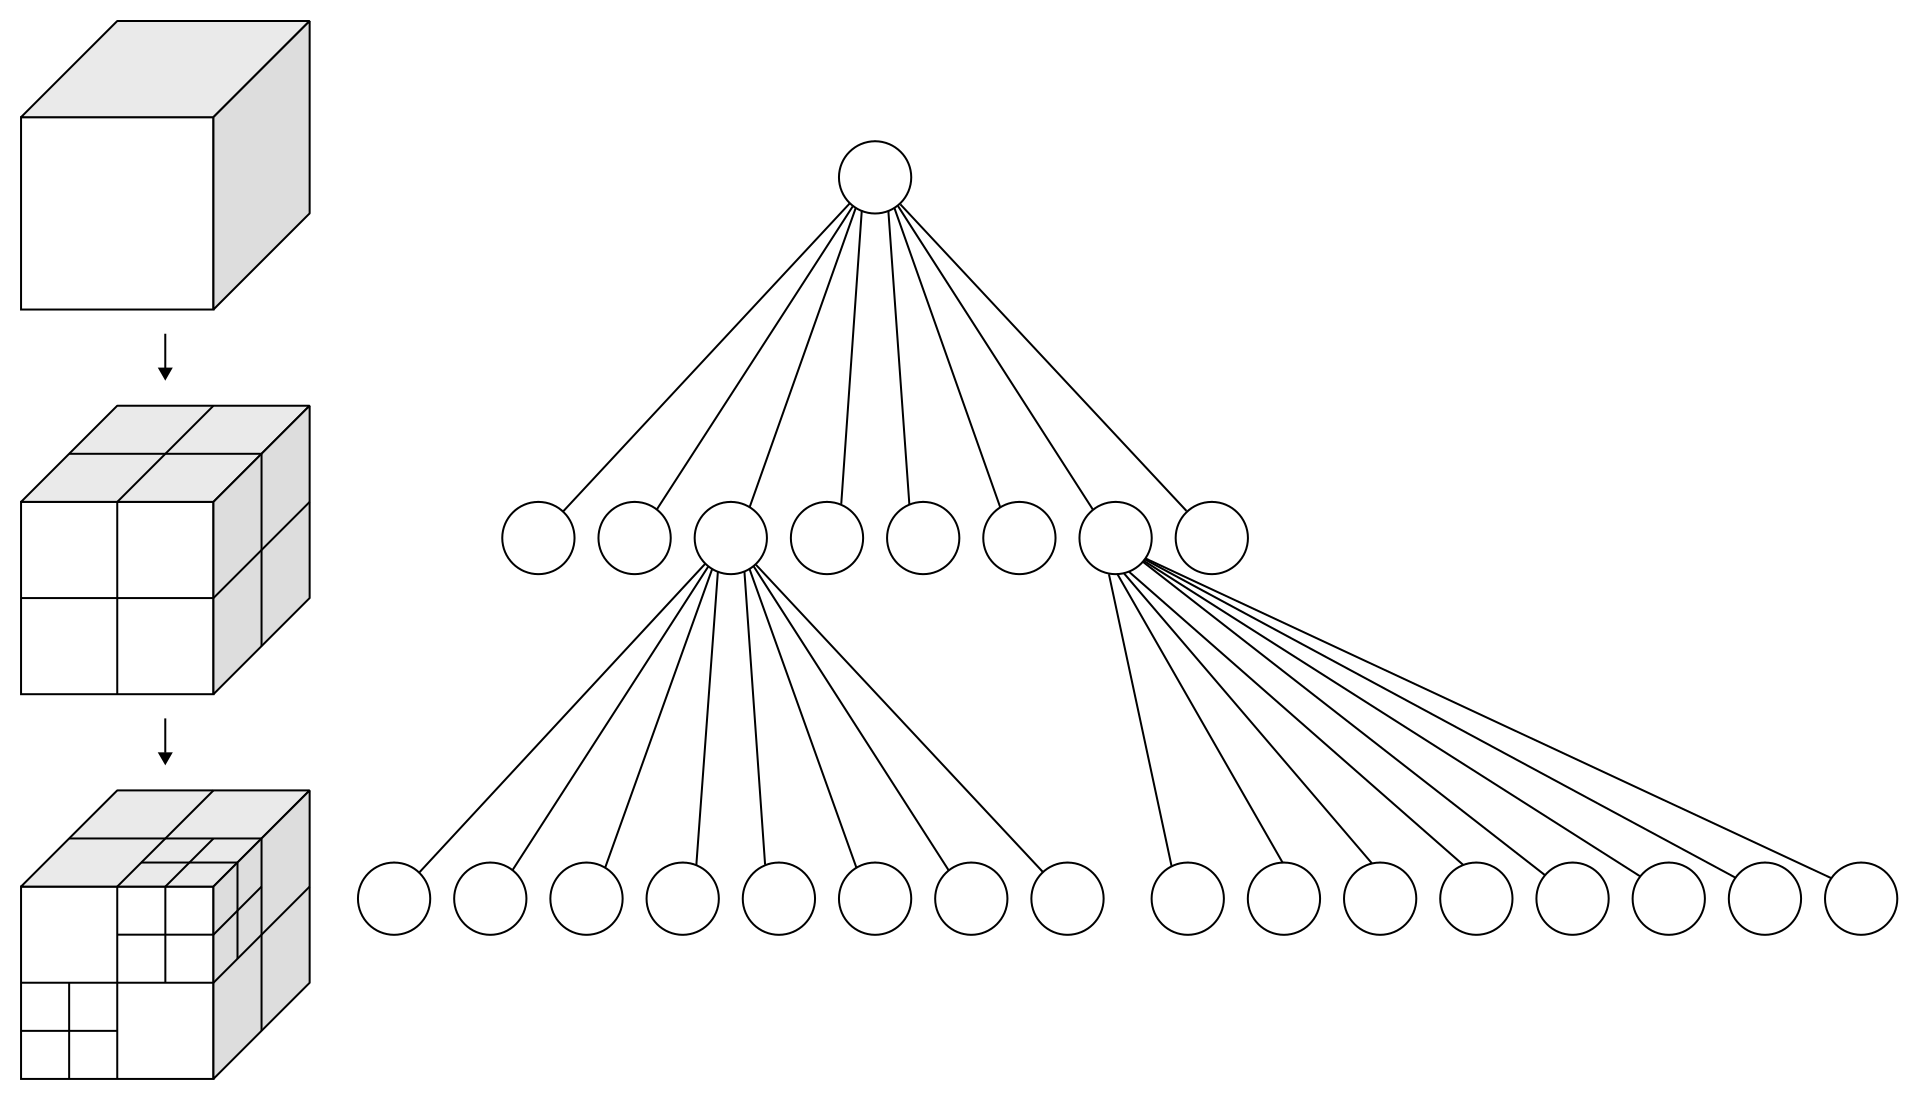
\includegraphics[scale=0.22]{octree.png}
	\end{center}
	\caption{Rekurzivno deljenje kocke na oktante.}
	\label{fig:oct}
\end{figure}



\section{Sweep and prune}
\label{subsec:sap}

Briši i odseci (eng. {\em sweep and prune}), skraćeno SAP, je alternativna tehnikama detekcije kolizije 
zasnovanim na prostornom particionisanju.
Sweep and prune je broadphase algoritam koji projektuje sve AABB
na bazne ose pa sortira sve projekcije da bi odredio preseke AABB.
Ako sve na sve tri ose projekcije para AABB seku, onda se i zaista u prostoru seče taj par AABB.
Ako je potreban samo jedan rezultat parova koji su u koliziji onda ovaj metod se ne ističe u odnosu na druge.
Moć sweep and prune algoritma je u tome što iskorišćava svojstvo temporalne koherencije.
Zbog toga je za svaku iteraciju potreban inkrementalan posao da bi se ažurirali parovi koji su u koliziji.
Objekti se ne teleportuju nasumično kroz prostor nego se postepeno kreću. 
Održavaju se tri sortirana niza, svaki je sadržan od $2n$ elemenata, gde je $n$ broj objekata.
Svaki niz sadrži sve projekcije AABB, po dva elementa za svaku projekciju. 
Jedan je početak, odnosno teme sa manjom koordinatom, a drugi je kraj projekcije, tj. teme sa većom koordinatom. 

Umesto da se vrše AABB upiti svaki put, moguće je da se čuvaju informacije o presecima 
na svakoj osi. To zahteva $O(n^2)$ memorije ali smanjuje posao prilikom zamena. \cite{sap}

Ovaj metod radi dobro kada su objekti dobro raspoređeni po većini osa, ali se loše pokazuje kada je
mnogo objekata zgusnuto duž jedne ose, što vodi kvadratnoj složenosti po broju objekata \cite{glavna2}.

\section{BSP}
\label{subsec:bsp}

% ==============================================================================
\chapter{Implementacija}
\label{sec:implementacija}
% ==============================================================================

Važno pitanje na početku ovog projekta je u kom okruženju ima najviše smisla da se implementira.
Tri glavna kandidata su OpenGL, Juniti (eng. {\em Unity}) i Anril Endžin (eng. {\em Unreal Engine}).

Unity i Unreal su oba pokretači igara, pa samim tim imaju sve što je neophodno da 
bi se krenuo ravoj igre ili neke druge aplikacije.
Unreal pruža mogućnost implementiranja preko shema (eng. {\em blueprints})
, preko programskog jezika C++ ili njihovom mešavinom.
Unity omogućava implementiranje pomoću programskog jezika C\# ili unityscript,
koji ima sintaksu nalik JavaSkriptu. Unityscript polako izlazi iz upotrebe, i 
sva nova dokumentacija podrazumeva korišćenje jezika C\#.
Jezik C\# u odnosu na C++ često omogućava kraće vreme implementacije nekog rešenja,
međutim postoji cena toga - nešto sporije vreme izvršavanja.
To "nešto" je uglavnom moguće ignorisati, prateći citat Donalda Knuta 
"Prevremena optimizacija je koren svog zla u programiranju".
Ipak, u slučaju programa čije performanse su od kritičnog značaja, npr. kao što je 
slučaj sa operativnim sistemima i pokretačima igara, to usporenje se ne može tolerisati.
%https://en.wikipedia.org/wiki/List_of_game_engines - kako referenca za ovo
Zato su danas praktično svi pokretači 3D igara implementirani u jeziku C++.

Upravo zbog svega što pokretači igara pružaju i njihove masivnosti nisu izabrani
za osnovu implementacije ovog projekta. Oni već imaju integrisanu fiziku, detekciju 
i razrešenje kolizije. Tako bi uobičajeni kanali implementacije u njima 
bili previše indirektni za funkcionalnost koja čini srž celog sistema.
Zbog navedenih razloga je projekat napravljen korišćenjem OpenGL pomoćne 
biblioteke FriGLUT (eng. {\em FreeGLUT}) koja ima skroman skup pomoćnih funkcija
funkcija, a od ostalih je većina usmerena na grafiku i vrlo su niskog nivoa.

Ovaj projekat ne implementira algoritme detekcije kolizije u izolaziji pošto 
se oni ni neće koristiti bez ostalih komponenti kao što su iscrtavanje, 
upravljanje ulazima korisnika, razrešenje kolizije, ažuriranje pozicije i brzine objekata.

\section{FriGLUT}

FriGLUT je alternativa otvorenog koda za GLUT (eng. {\em OpenGL Utility Toolkit}). 
GLUT je prvobitno napisan da bi se podržali primeri programa u knjizi "OpenGL:
vodič za programiranje", poznatija pod nazivom "Crvena Knjiga" (eng. {\em "the Red Book" }).
GLUT se ne razvija od 1998. godine, pa je još 1999. započet FriGLUT projekat koji 
se razvija do danas. 
\cite{freeglut}

FriGLUT se stara o pravljenju prozora, obrađivanju događaja kroz glavnu petlju,
a i zajedno sa njim su dostupne i standardne funkcije OpenGL-a koje se koriste
za iscrtavanje poput glTranslatef, glScalef, glLightf, glMaterialfv, glViewPort, itd.
Za odgovore na događaje pritiskanja tastera, puštanja tastera i pomeraja miša
FriGLUT propisuje korišćenje funkcija povratnog poziva  (eng. {\em callbacks }) koje je potrebno implementirati.
FriGLUT se ne stara o tome da li je u nekom trenutku neko dugme pritisnuto, 
koliki je pomeraj miša, niti ga automatski repozicionira, ali barem pruža 
funkcije koje su neophodne da bi se to ostvarilo.

\section{Arhitektura}

Glavne komponente programa su:
\begin{itemize}
	\item Komponenta za iscrtavanje
	\item Komponenta za rukovanje ulazima korisnika
	\item Centralna komponenta - poziva sve ostale komponente i stara se o vremenskim koracima
	\item Kontroler komponenta za upravljanje svim parametrima algoritama
	\item Komponenta za merenje performansi
	\item Komponenta za ažuriranje brzine i pozicije objekata
\end{itemize}

\begin{figure}[h!]
	\centerfloat
% https://online.visual-paradigm.com/w/jllvezfo/diagrams.jsp#diagramlist:open&mode=Local
	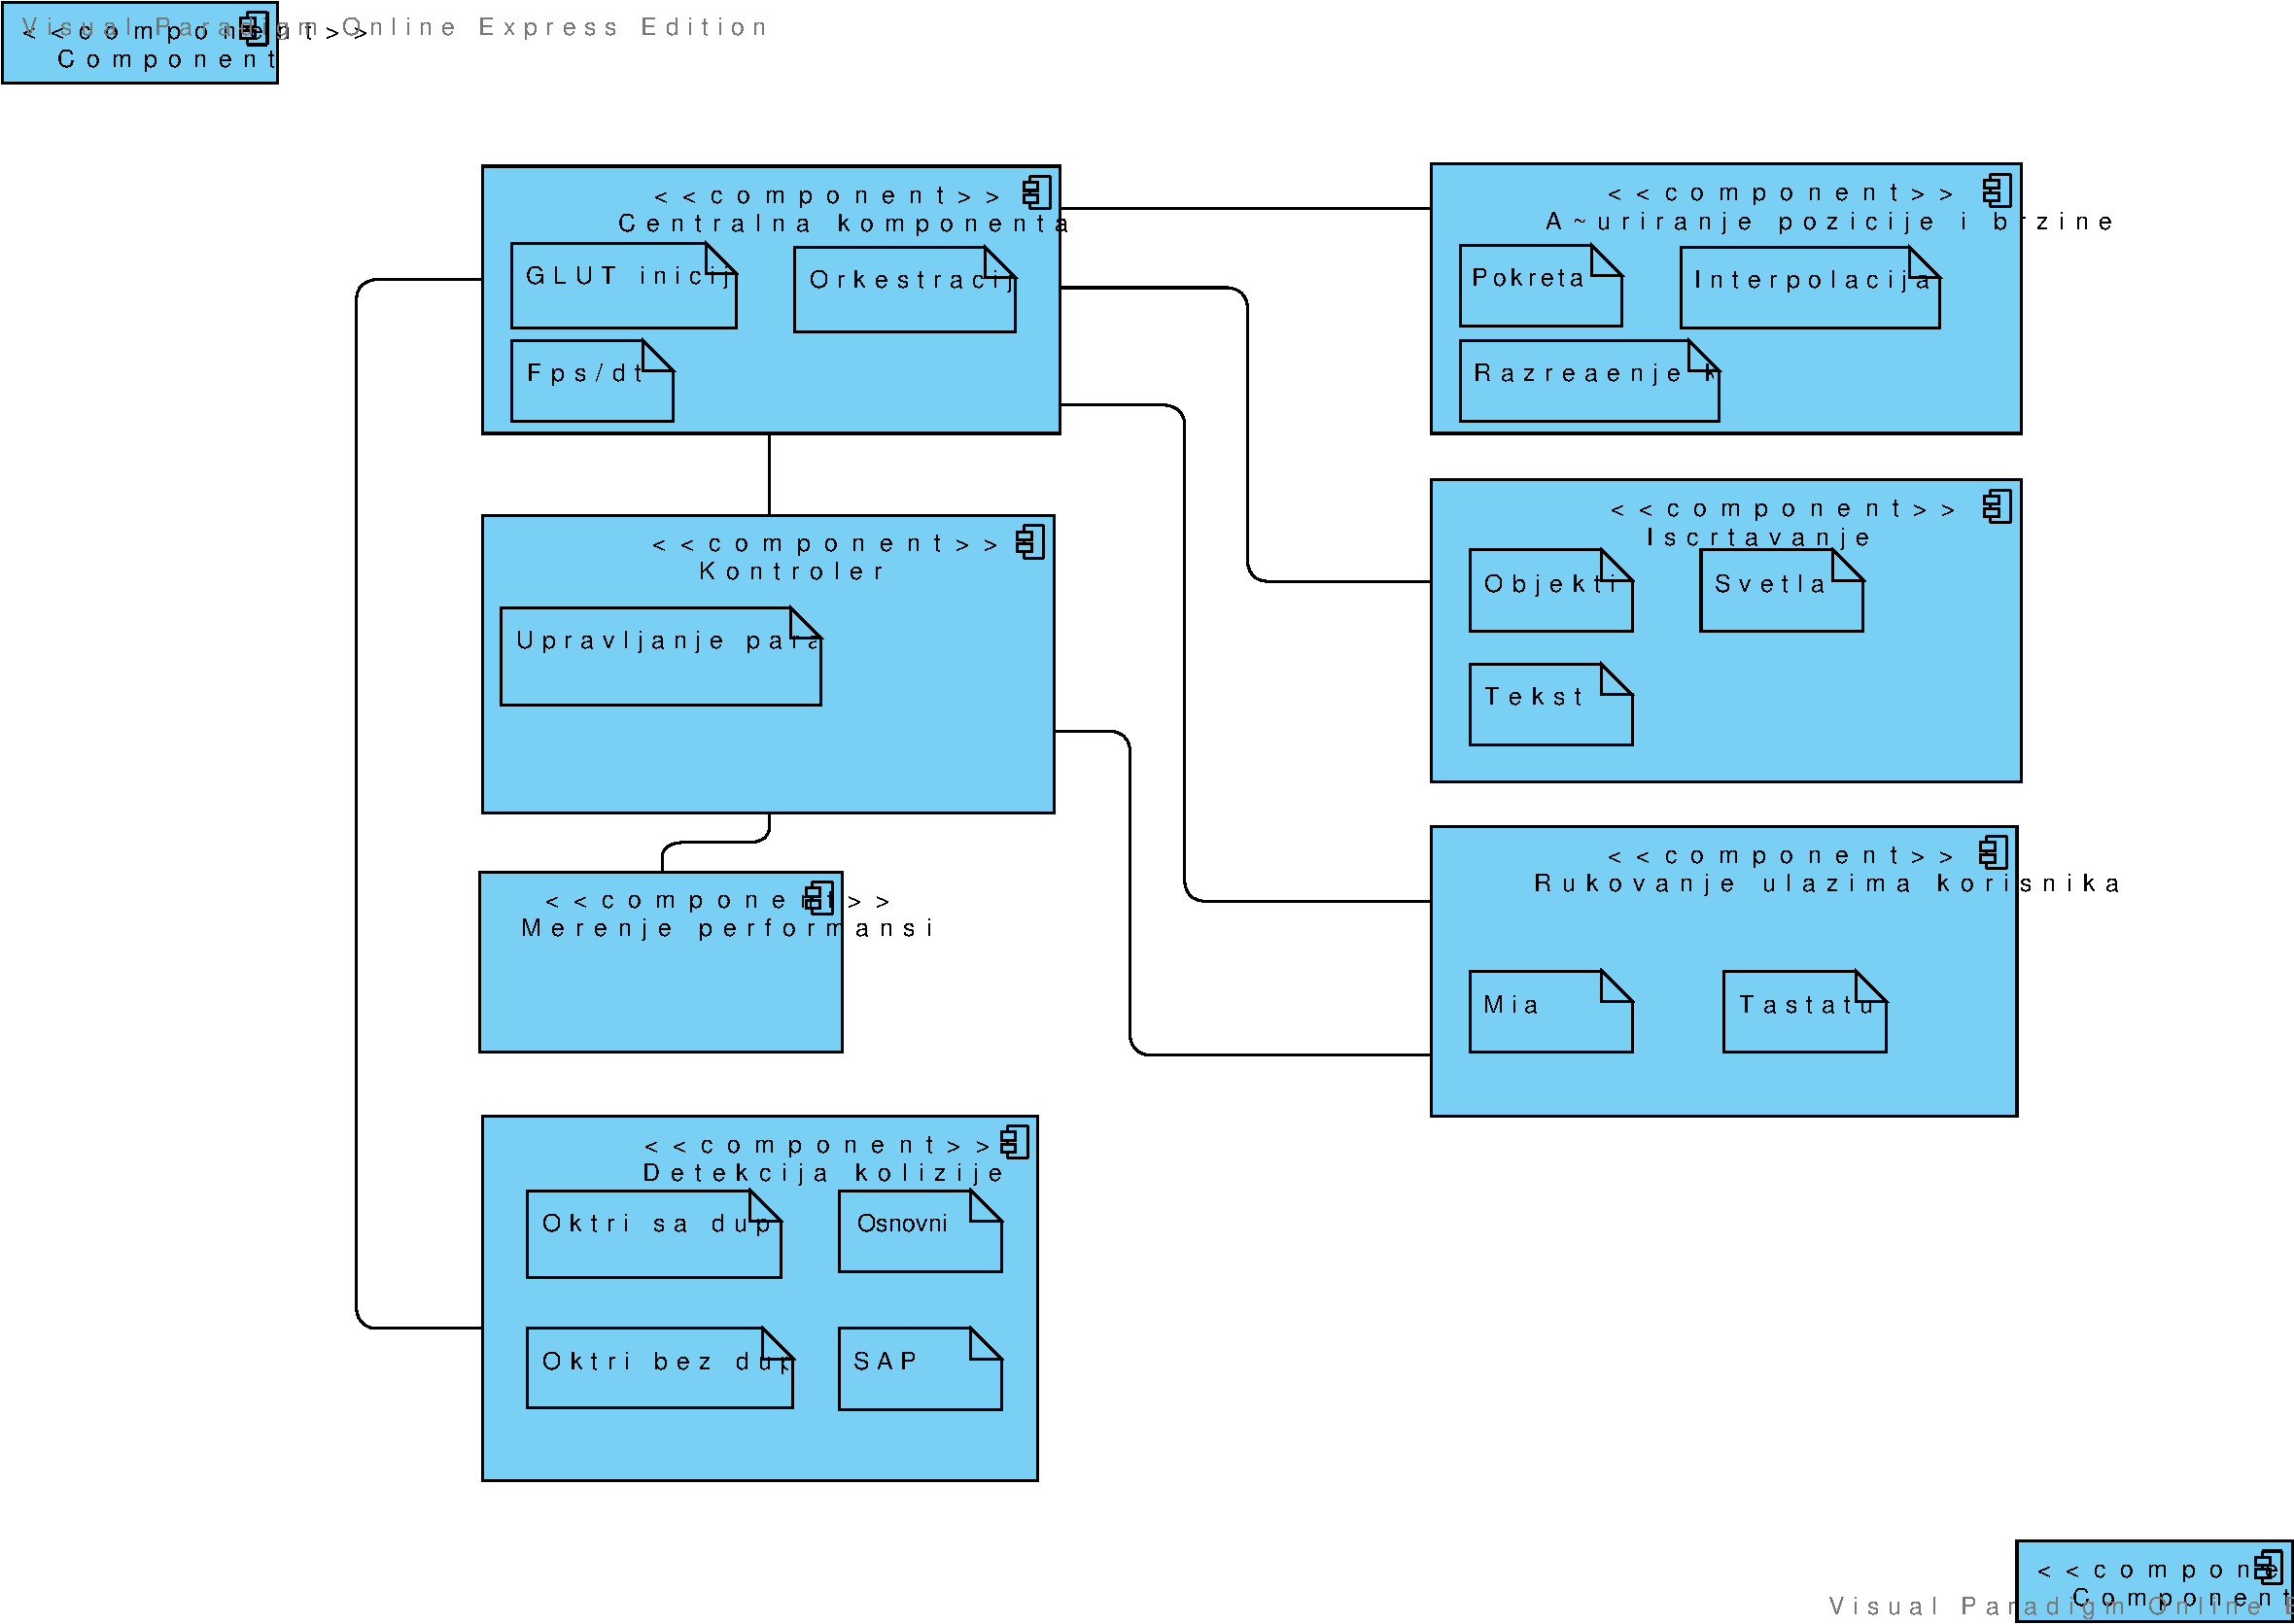
\includegraphics[trim=150 50 100 50,clip,scale=0.6]{architecture.pdf}
	\caption{Arhitektura.}
	\label{fig:archi}
\end{figure}

Na slici \ref{fig:archi} je prikazana arhitektura programa sa navedenim komponentama.

\subsection{Kontroler komponenta}

Parametri koji se menjaju kroz kontroler komponentu su: 
\begin{itemize}  
	\item Broj objekata koji su podložni koliziji. 
	Ovo je parametar koji svakako najviše utiče na ponašanje algoritama.
	\item Veličina objekata. 
	Na prvi pogled liči da ne bi mnogo uticalo na perofmanse, međutim veliki objekti u malom prostoru mogu katastrofalno usporiti izvršavanje.
	\item Brzina kretanja objekata.
	Ovaj faktor ne utiče na mnoge algoritme, ali je u slučaju SAP algoritma najbitniji. Može promeniti odlično ponašanje SAP algoritma u slučaju sporog kretanja 
	objekata i učiniti ga praktično algoritmom kvadratne složenosti u najgorem slučaju.
	\item Veličina kontejnera u kome se nalaze i kreću svi objekti.
	Daje još jednu perspektivu kako veličina objekata i odnos te veličine sa celim prostorom, ovde kontejnerom, utiču na performanse.
	\item Maksimalan broj elemenata u listu Oktrija.
	Promena maksimalnog broja elemenata u listu pre nego što se on podeli na podoktante utiče "samo" na konstantan faktor vremenske složenosti.
	To uopšte nije zanemarljivo u datom kontekstu i povoljnosti koje daje povoljno izabran parametar su vrlo vidne.
	\item Maksimalna dubina Oktrija. Što veća dubina je uglavnom povoljnija, mada treba biti oprezan ako se može desiti 
	da se velik broj objekata preklapa unutar jednog oktanta, jer se tada samo gubi vreme i troši dodatna memorija. 
	Pokušavaju se razdvojiti objekti rekurzivnom podelom potprostora, ali pošto se oni presecaju taj put je beznatežan.
	\item Da li raditi razrešenje kolizije. 
	Razrešenje kolizije je odvojen problem od detekcije kolizije, a pošto se uglavnom koriste oba, onda je dobro videti 
	kako razrešenje kolizije deluje na performanse detekcije kolizije. Praktično uvek deluje povoljno, pošto onemogućava da se mnogo 
	objekata međusobno preseca, pa time smanjuje verovatnoću da se stvori veliki klaster objekata koji bi usporio izvršavanje.
	\item Koji algoritam detekcije kolizije se koristi. Podržani su: osnovni (trivijalni) algoritam, Oktri sa duplikatima,
	Oktri bez duplikata i SAP algoritam. Takođe je moguće isključiti detekciju kolizije u celosti da bi se dobila referntna vrednost vremena izvršavanja.

\end{itemize}  

Kontroler komponenta takođe pruža mogućnost menjanja pravca kretanja objekata. 
Tada svi objekti bivaju usmereni prema trenutnoj poziciji posmatrača. 
Potrebna je takva funkcionalnost pošto ona povećava koncentraciju objekata, 
pogotovo nakon što se odbiju o ivicu kontejnera. Tada će se većina objekata 
naći oko centra kontejnera, što dovodi do eksplozije vremena izvršavanja, pogotovo u slučaju Oktrija sa duplikatima.

\subsection{Komponenta za iscrtavanje}

Sve što se želi prikazati mora se iskazati preko GL funkcija. 
Boje objekata zavise od osvetljenja i materijala ili teksture koja mu je dodeljena.

Ljudska percepcija boje objekta je zapravo spektar elektromagnetnog zračenja koji se odbija o taj objekat i pada na retinu oka.
U pravom svetu se zraci svetlosti odbijaju od više objekata pre nego što stignu do oka. 
Simulacija takvog ponašanja se naziva praćenje svetlosti (eng. {\em raytracing}).  
Praćenje svetlosti je računarski zahtevno, pa do skoro nije bilo moguće izvršavati ga u realnom vremenu, već samo na farmi servera koji renderuju neku scenu.
2018. godine je firma Nvidia pustila u prodaju novu seriju grafičkih karti koje hardverski implementiraju praćenje svetlosti. 
U trenutku pisanja se ova tehnologija koristi kao hibrid, odnosno ne kao zamena nego dopuna postojećih metoda.

Uobičajeno je da se materijali objekata opisuju pomoću Fongovog modela senčenja. 
Fongov model je empirijski model osvetljenja. Razvio ga je Bui Tuong Fong i objavio ga u svojoj doktorskoj tezi 1975. godine.
Opisuje boju površi kao kombinaciju difuzne refleksije, tj. odbijanja svetlosti sa grubih površi, 
spekularne refleksije, tj. refleksija sa sjajnih površi, i ambijantne refleksije, koja predstavlja manju količinu svetlosti 
koja je raspršena kroz celu scenu.
\cite{Phong} OpenGL nudi Fongov model pa se on koristi za opisivanje materijala svih objekata.
Todo slika možda.
Uključeno je jedno globalno svetlo, a moguće je da posmatrač postavi jos najviše osam svetala na 
proizvoljne statične blokove na mapi.
Komponenta se brine i o iscrtavanju teksta, što zahteva nešto više gl poziva nego što bi se očekivalo.
Postavljanje kamere zavisi od pozicije posmatrača i njegovog usmerenja pogleda levo-desno i gore-dole.
Kamera se usmerava od pozicije posmatrača ka pravcu u kome gleda.
Vektor pravca gledanja se dobija prema formuli:

\begin{equation}
\label{eq:camera}
\begin{split}
x = cos(hrot) \cdot cos(vrot) \\
y = sin(vrot) \\
z = cos(hrot) \cdot  cos(vrot)	
\end{split}
\end{equation}


Gde je $vrot$ ugao između $xz$ ravni i pravca gledanja, dok je $hrot$ ugao rotacije oko $y$ ose.
Napomena da je u OpenGL-u $y$ osa vertikalna, $x$ horizontalna, a $z$ predstavlja dubinu.


\subsection{Centralna komponenta}

Centralna komponenta inicijalizuje GLUT funkcije povratnog poziva, postavlja GL parametre, i pokreće sistem.
Definiše tajmer koji će periodično pozivati ažuriranje sistema i zakazati njegovo ponovno iscrtavanje. 
Stara se o računanju vremena dva uzastopna koraka izvršavanja, redosledu pozivanja ažuriranja stanja,
detekcije kolizije, razrešavanja kolizije i iscrtavanja.

\subsection{Komponenta za ažuriranje brzine i pozicije objekata}
% ona radi i razresavanje kolizije

Svaki objekat sadrži trojku brojeva u pokretnom zarezu koja označava njegovu poziciju za svaku koordinatu prostora.
Za održavanje pravca je potrebna još jedna trojka koja predstavlja vektor brzine kretanja.
Ako se pritom želi da objekat postepeno ubrzava kada se primeni sila na njega, ili da postepeno usporava 
kada prestane delovanje sile, onda se mora čuvati još jedna trojka brojeva, koja predstavlja ciljnu brzinu.
Postepeno ubrzavanje se koristi prilikom upravljanja posmatrača. 
Kada se pritisne dugme na tastaturi za pomeranje posmatrača, očekivano ponašanje je da neće istog trenutka 
početi da se kreće maksimalnom brzinom, već postepeno da ubrzava.
Isto, kada se pusti dugme, "sila" koja je delovala na posmatrača je nestala, ali je on imao momentum pa će
nastaviti malo napred.

Potrebno je posvetiti pažnju kako se posmatrač kreće na komandu da ide napred-nazad ili levo-desno.
Prva ideja bi bila da se za kretanje levo-desno poveća ili smanji vrednost pozicije $x$ koordinate posmatrača,
ili da se menja $z$ koordinata posmatrača kada treba da se kreće napred-nazad.
To ipak nije dobro rešenje pošto kada neko želi da se pomeri ne razmišlja preko strana sveta na koju će stranu, 
već relativno u odnosu na trenutnu njegovo usmerenje. Usmerenje je dato formulom \ref{eq:camera}.
Neka je dat trodimenzioni vektor $v$ koji predstavlja usmerenje pogleda, tada je vektor 
kretanja unapred jednak: 
$$ v_{napred} = \frac{(v_1, 0, v_2)^T}{||(v_1, 0, v_2)^T||} $$
Pritom se normira vektor kako se ne bi sporije kretalo u slučaju gledanja gore ili dole, 
pošto su tada $v_1$ i $v_2$ mali.
Slično, vektor kretanja u stranu se računa kao:
$$ v_{bok} = \frac{(-v_2, 0, v_1)^T}{||(-v_2, 0, v_1)^T||} $$

Sada su zamenjene vrednosti prvog i trećeg elementa vektora zato što kada se gleda pravo u smeru $x$ ose, 
onda je bočno kretanje duž $z$ ose. Razlog za promenu znaka $v_2$ je jednostavno zbog orijentacije $z$ ose u odnosu na $xz$ ravan.
% todo negde ubaci sliku koordinatnog sistema opengla

% ==============================================================================
\chapter{Evaluacija}
\label{sec:evaluacija}
% ==============================================================================

Merenja vremena izvršavanja i memorije u zavisnosti od algoritma i parametara.
Grafici i parelele sa prethodno opisanim principima.




% ==============================================================================
\chapter{Zaključak}
\label{sec:zakljucak}
% ==============================================================================

Zaključak. 

% \addcontentsline{toc}{section}{Literatura}
% \appendix
% \bibliography{bibl} 
% \bibliographystyle{plain}


% ------------------------------------------------------------------------------
% Literatura
% ------------------------------------------------------------------------------
\literatura

% ==============================================================================
% Završni deo teze i prilozi
\backmatter
% ==============================================================================



% \appendix
% \section{Dodatak}
% Dodatak.

\end{document}
